
The simple model we saw in the previous section is an example of discrete dynamical systems. Now we move on to a slightly more complicated case. The radius of a tumor increases at a rate of  15 \% every hour, what is the doubling time of the tumor? The general form of equation \ref{geomgrowth_example} for a growth rate $r$ is:

\begin{equation}
\label{geomgrowth_general}
x_{t+1} = x_t  + r \, x_t =(1 + r) \, x_t
\end{equation}

and so

\begin{equation}
\label{geomgrowth_general2}
x_{t} = (1 + r)^{t} \, x_0
\end{equation}


this is called \textbf{geometric growth} with growth rate $r=0.15$ for our tumor. 



Biologists often describe growth using its doubling time, $t_d$,  which is the time needed for the system to duplicate its size. So if our tumor starts with size $x_0$, it will become double after a time $t_d$:

\begin{equation}
2\, x_{0} = (1 + r)^{t_d} \, x_0
\end{equation}

where $x_0$ cancels out. Now we can take  logarithms and rearrange:

\begin{equation}
t_d = \frac{\log 2}{\log (1 + r) }
\end{equation}

So our doubling time for $r=0.15$ is 1.74 hours, about an hour and 45 min.

\section{Dealing with many things at once: vectors and matrices}

The  individuals in a population are not always identical. Most of the time, biological populations have many different types of individuals. Cells differentiate into types, animals grow in different stages, microbes can form spores \dots Fortunately, we have the mathematical tools to reflect that diversity. Consider a population of parasites that reproduce through eggs. Every week, some eggs hatch and produce new parasites that in time will produce more eggs. We can easily capture the idea of our population having two different individuals: eggs, $x_1$ and animals, $x_2$. When we want to refer to all individuals of the species, regardless of their type, we will use vector $\mathbf{x}$.

\begin{equation}
\mathbf{x} =\left( \begin{array}{c} x_1 \\  x_2 \end{array} \right)
\end{equation}

A vector of dimension $n$ is just a collection of $n$ ``ordinary'' numbers which, by the way, are called scalars. So the total population is represented by vector  $\mathbf{x}$, which is composed of $x_1$ eggs and $x_2$ animals. We write vectors and matrices (see below) in \textbf{boldface}.


When we study the dynamics of this population, we will see why it was so important to keep the two types separate. The number of eggs produced each generation does not depend on the number of eggs present in it. Eggs are laid by the animals, so the more animals there are, the more eggs are produced:

\begin{equation}
x_1 = f_{1} \,  x_2 
\end{equation}

where $f_1$ is the fecundity of the animals ($x_2$). The production of new animals is also dependent of the fraction of eggs that survive the incubation period so for a survival ratio $s_1$:

\begin{equation}
	x_2 = s_{1} \,  x_1 
\end{equation}

In this simple case, we can just work with the two equations, but as the complexity of the population increases, we have to find a more efficient method to handle the complex interactions between all the groups. Lets assume we are studying a population of mice with three different age groups: young  mice up to one year old, $n_1$, can reproduce at very low rates, mice between 1 and 1.5 years old, $n_2$, are adults in their prime and old mice up to two years old, $n_3$, have more fragile health, which leads to lower fecundity. We can summarize this information making a drawing, as shown in figure \ref{fig:mice}. Each age group is represented by a circle, and each process changing the population, by an arrow. The starting point of an arrow shows which group determines the speed of the process while the  destination of the arrow shows which group is affected by it.

\begin{marginfigure}
	\begin{center}
		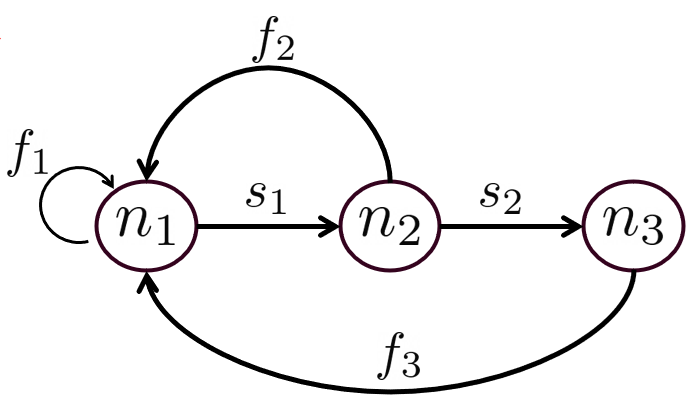
\includegraphics[width=0.9\textwidth]{Mouse_pop_graph}
	\end{center}
	\caption{Dynamics of a population of mice. Circles contain the three age groups that are connected by arrows showing how one population affects the growth of another. Symbols on top of each arrow show the coefficient that governs the interaction. For instance, $f_3$ is the fecundity of old mice, $n_3$, while $s_1$ is the fraction of young mice that survive to adulthood.}
	\label{fig:mice}
\end{marginfigure}
 
The figures show clearly that the increase in young mice, $n_1$, for each generation will depend on the fecundities of all three age groups, while the growth of old mice $n_3$, only depends on the survival of adult mice $n_2$. The arrows clearly show which population affects which but, how do we write our equations? Fortunately, mathematics has a simple tool to transform drawings into numbers: matrices.

A matrix is just a square of numbers that connects elements represented in its columns to elements represented in its rows. Since our drawing connects the three elements $n_1$, $n_2$, $n_2$ to one another, we will have a row and a column for each. Lets start making such a square and fill it with zeros:

\begin{center}
\begin{tabular}{c|ccc}
	& $n_1$ & $n_2$ & $n_3$ \\
	\hline 
	$n_1$ &0	&0	&0	\\
	$n_2$ &0	&0	&0	\\
	$n_3$ &0	&0	&0	\\
\end{tabular}
\end{center}

And now, we will place a number for each arrow in the drawing. The starting point of the arrow will be the column where we place the number and the ending point of the arrow will be the row. Our table will look like this.

\begin{center}
	\begin{tabular}{c|ccc}
		& $n_1$ & $n_2$ & $n_3$ \\
		\hline
		$n_1$ &$f_1$	&$f_2$	&$f_3$	\\
		$n_2$ &$s_1$	&0	&0	\\
		$n_3$ &0	&$s_2$	&0	\\
	\end{tabular}
\end{center}

So the fecundity $f_3$ connects $n_3$ (column) to $n_1$ (row) and so on. We do not Normally use the titles for row and columns, so we would write our matrix as:

\begin{equation}
\mathbf{L} =	\begin{pmatrix}
		f_1	&f_2	&f_3	\\
		s_1	&0	&0	\\
		0	&s_2	&0
	\end{pmatrix}
\end{equation}

Now it is very easy to get the equations, since vectors and matrices have their own mathematical operations. The transition from one vector to another ( $n_t \mapsto n_{t+1}$ ) Is obtained by multiplying the initial vector:

\begin{equation}
	\mathbf{n_{t+1}} =\mathbf{L} \cdot \mathbf{n_t}
	\label{fig:matequationL}
\end{equation}

The matrix $\mathbf{L}$ is commonly known as the Leslie matrix to honor Patrick H. Leslie, the ecologist who proposed it. If we now apply the product between vectors and matrices as we learned in high school, we will see that:

\begin{equation}
	 	\begin{pmatrix}
		f_1	&f_2	&f_3	\\
		s_1	&0	&0	\\
		0	&s_2	&0
	\end{pmatrix} \cdot \begin{pmatrix} n_{1,t}\\ n_{2,t} \\ n_{3,t}\end{pmatrix} = \begin{pmatrix} f_1 \,n_{1,t} + f_2 \,n_{2,t} + f_3 \,n_{3,t}\\ s_1 \, n_{1,t} \\ s_2 \, n_{2,t}\end{pmatrix}
\end{equation}

and we can apply our growth equation as many times as we want:

\begin{equation}
	\mathbf{n_{2}} =\mathbf{L} \cdot \mathbf{n_1} = \mathbf{L} \cdot \mathbf{L} \cdot \mathbf{n_0} 
\end{equation}

and for $k$ generations:

\begin{equation}
	\mathbf{n_k} =\mathbf{L}^k \cdot \mathbf{n_0}
\end{equation}

where $\mathbf{L}^k$ mans we multiply the matrix by itself $k$ times.

Equation \ref{fig:matequationL} shows a very useful fact.  By multiplying a vector times a matrix, we \emph{transform} this vector into another. For this reason, we often talk about a matrix as a \textbf{transformation}.  Here we use matrix $\mathbf{L}$ it to transform the current population into the population of the next generation. When we represent anything by a vector -- e.g the direction and intensity of a ray of light -- we can represent changes in ts state by a matrix multiplication --e.g. the direction and intensity of the light after passing through liquid medium. This capacity of abstraction is what makes mathematics so powerful in science and engineering. Solving a problem once in a field like physics means solving hundreds of problems in other fields.

Back to our population of animals, we may wonder how it is going to change in the future.  Is the age distribution of the population going to stabilize in the long run or will it keep changing forever? This kind of questions are also very relevant for economists and social scientists. Will the population of developed countries continue to get older? Or will the aging stop at some point? The solution to this question is important since all our pensions depend on it. Surprisingly enough, the answer was already found in the 18$^{th}$ century by Leonard Euler while he was working on a completely different problem: the rotation of rigid bodies.

\section{Eigenvalues and eigenvectors}

Back to our mice example, look at the behavior of our population along several generations in figure~\ref{fig:Lpop}.

\begin{figure*}
\begin{center}
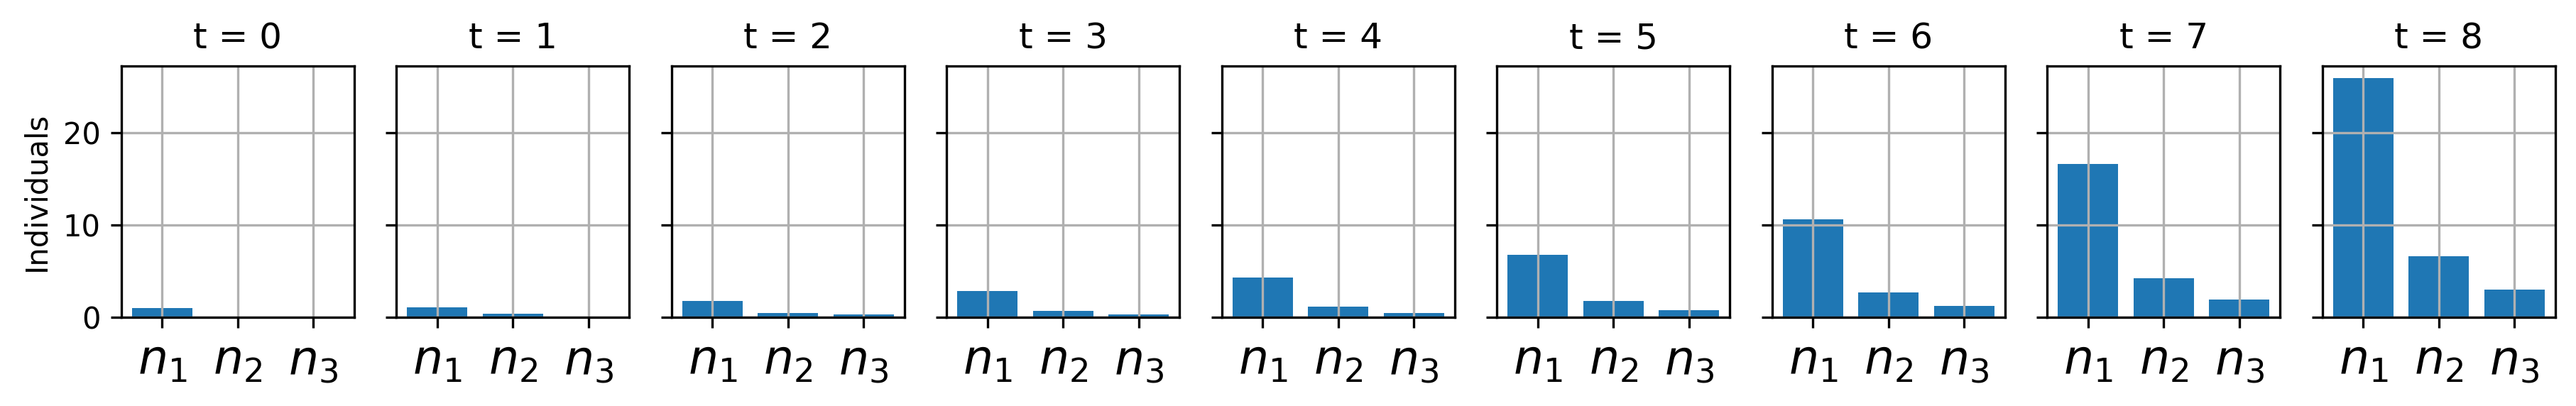
\includegraphics[width=\linewidth]{pop_evol}
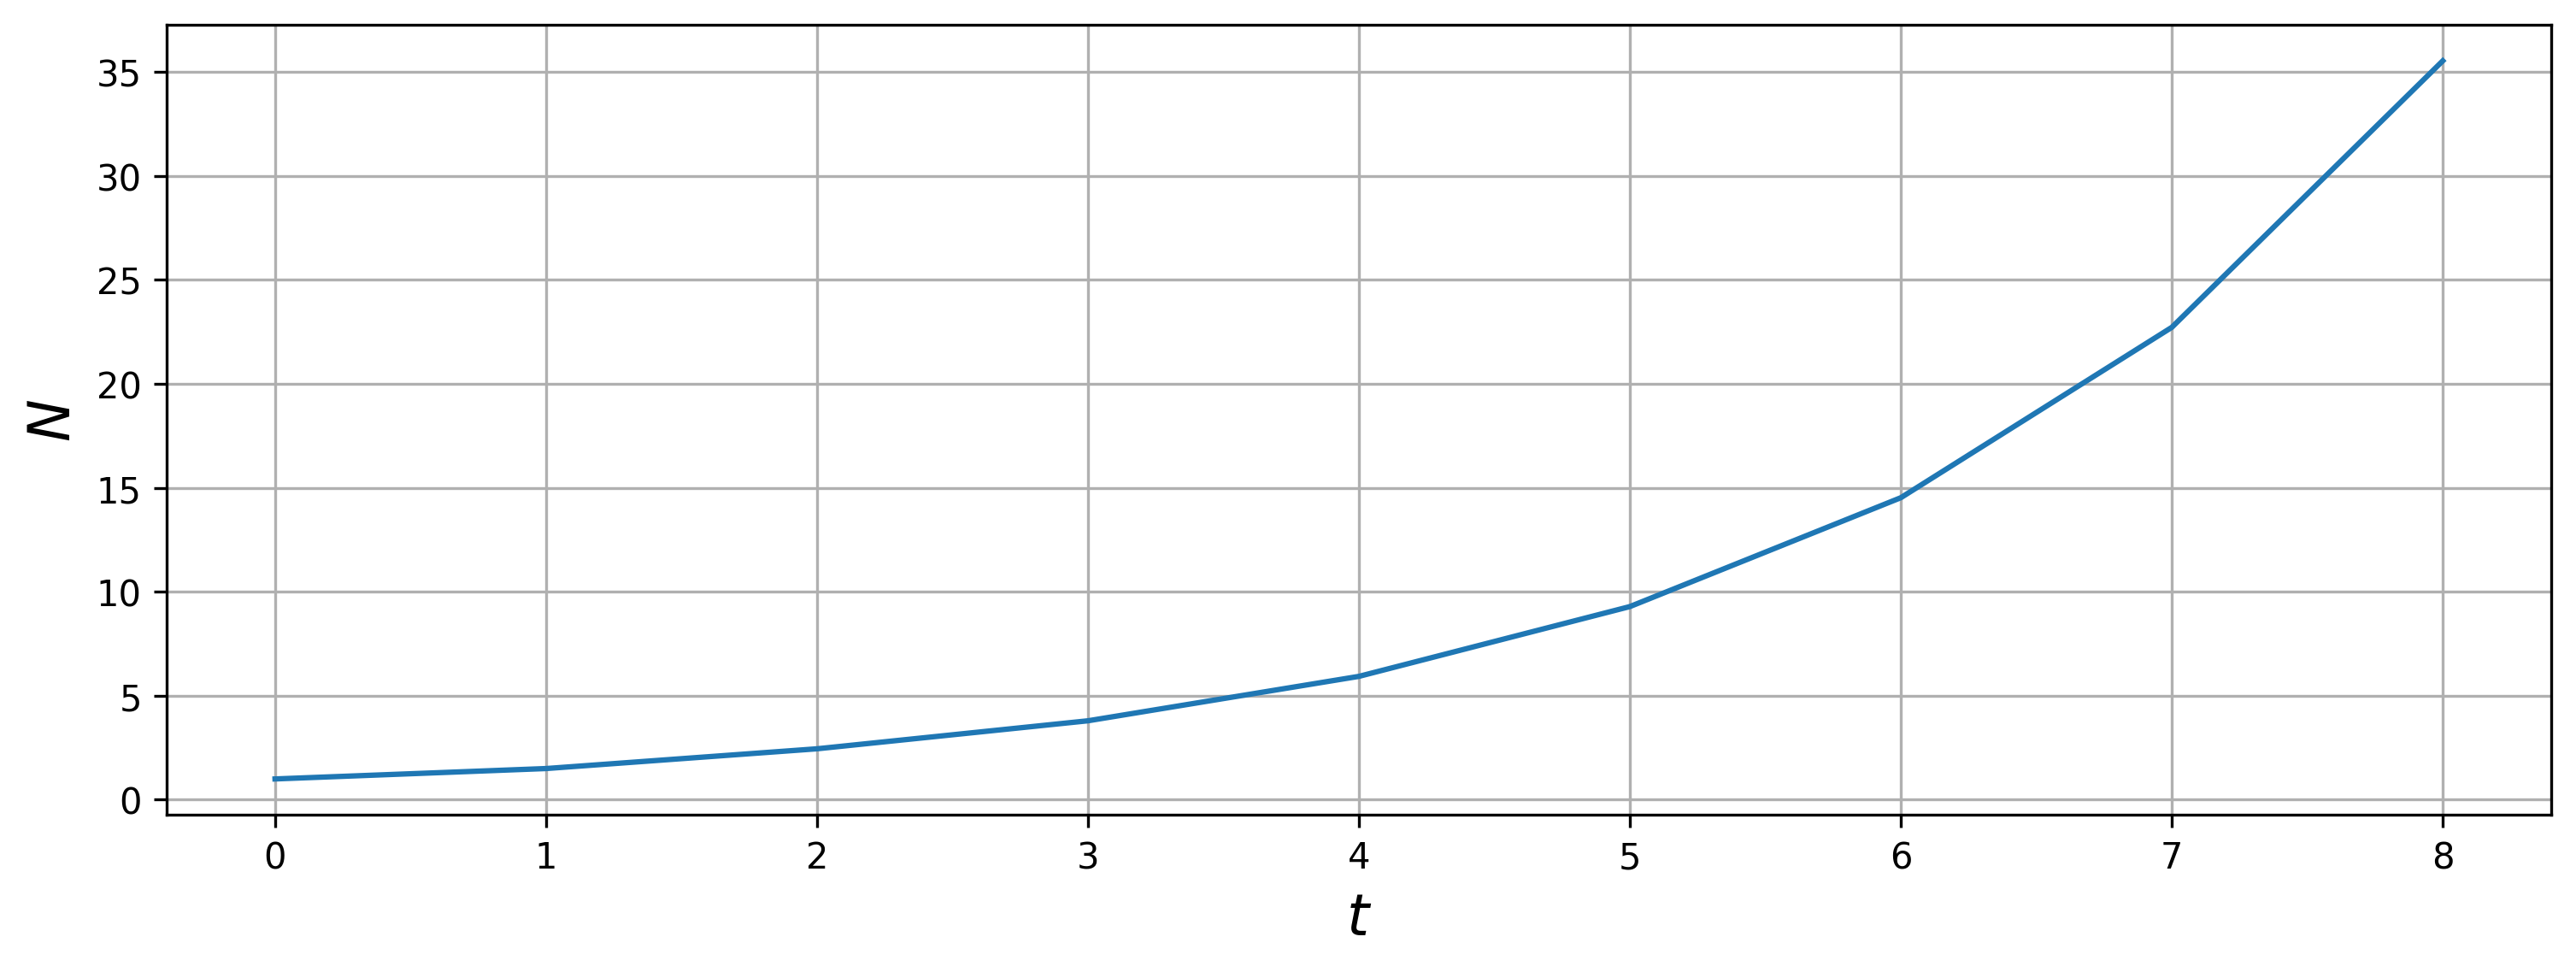
\includegraphics[width=\linewidth]{tot_pop_evol}		
\end{center}
\caption{The upper graph shows the population structure as a bar graph for nine generations. The figure below shows the total population for each generation (the sum of all three age groups). As the total population increases, it is obvious that the vector is different each generation, but the proportion of the three age groups, seems to be very similar for each generation.}
\label{fig:Lpop}
\end{figure*}




The population keeps growing, so the vectors keep changing, but looking at their shape, it looks like it is well preserved from one generation to the next. There are always more young mice than adults and more adults than seniors. Does this mean the population will reach a stable age structure?

Imagine that the vectors of the population for several consecutive generations are as follows:

\begin{equation}
	n_0 = \begin{pmatrix} 3\\ 2 \\ 1\end{pmatrix}, 
	n_1 = \begin{pmatrix} 6\\ 4 \\ 2\end{pmatrix}, 
	n_2 = \begin{pmatrix} 12\\ 8 \\ 4\end{pmatrix}
\end{equation}

It is easy to see that $\mathbf{n_1} = 2 \cdot \mathbf{n_0}$  and $\mathbf{n_2} = 2 \cdot \mathbf{n_1}$. In other words, the matrix preserves the ``shape'' of the vector and just increases its size.

\begin{equation}
 \begin{pmatrix} 6\\ 4 \\ 2\end{pmatrix} =  2 \cdot\begin{pmatrix} 3\\ 2 \\ 1\end{pmatrix} 
 \label{eigenvect_in_action}
\end{equation}

This means our population will keep growing -- in this case, it will double its size every generation -- but the age structure will remain stable with three young mice for every two adults and one senior. In fact, we could have made this prediction just looking at the matrix $\mathbf{L}$. Every matrix has a few vectors that keep their direction when transformed by it. They may become longer or shorter, because they are multiplied by a certain scalar. This property is so important in science and engineering that it has a formal definition we should learn. Given matrix $\mathbf{A}$, we say $\mathbf{v}$ is an eigenvector of  $\mathbf{A}$ if:
 
\begin{equation}
	\label{eigendefinition}
	\mathbf{A} \, \mathbf{v}  = \lambda  \,	\mathbf{v}   
\end{equation}

The number $\lambda$ is a scalar associated to that particular eigenvector and it is called an eigenvalue. In the example shown in equation \ref{eigenvect_in_action}, $(3,2,1)$ would be an eigenvector and $2$ would be its corresponding eigenvalue.

Every matrix of dimensions $n \times n$ has exactly $n$ eigenvectors and $n$ eigenvalues. Eigenvectors can be understood as the natural "axes" to study the transformation. If our coordinates are aligned with the eigenvectors, we can understand any transformation as just ``stretching'' or ``shrinking'' the vector in each direction by the corresponding eigenvalue. For instance, the matrix

\begin{equation}
	\mathbf{A}=\begin{pmatrix} 0.5 & 0\\ 0 &  2 \end{pmatrix} 
\end{equation}

has dimension $2 \times 2$, so it has two eigenvectors with their corresponding eigenvalues. one eigenvector is $\mathbf{v_1}=\begin{pmatrix}  0\\ 1 \end{pmatrix} $,  -- that goes along the y-axis -- and its corresponding eigenvalue is $\lambda_1 = 2$. multiplying the matrix times $\mathbf{v_1}$, proves it is indeed an eigenvector with eigenvalue 2:

\begin{equation}
	\begin{pmatrix} 0.5 & 0\\ 0 &  2 \end{pmatrix} \cdot \begin{pmatrix}  0\\ 1 \end{pmatrix} = \begin{pmatrix}  0\\ 2 \end{pmatrix}= 2 \, \begin{pmatrix}  0\\ 1 \end{pmatrix}
\end{equation}

The same happens with the second eigenvector $\mathbf{v_2}=\begin{pmatrix}  1\\ 0 \end{pmatrix}$ -- on the x-axis --, which has eigenvalue $\lambda_2 = 0.5$.

\begin{equation}
	\begin{pmatrix} 0.5 & 0\\ 0 &  2 \end{pmatrix} \cdot \begin{pmatrix}  1\\ 0 \end{pmatrix} = \begin{pmatrix}  0.5\\ 0 \end{pmatrix}= 0.5 \, \begin{pmatrix}  1\\ 0 \end{pmatrix}
\end{equation}

\begin{marginfigure}
	\begin{center}
		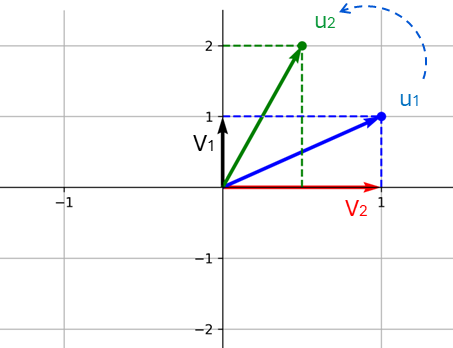
\includegraphics[width=0.9\textwidth]{transform}	
	\end{center}
	\caption{Role of eigenvalues in a matrix transformation. The black eigenvector $\mathbf{v_1} = (0,1)$ has eigenvalue 2 while the red eigenvector $\mathbf{v2}=(1,0)$ has eigenvalue 0.5. When a vector like $\mathbf{u_1}$ -- in blue -- is transformed, it just gets stretched twice in the vertical axis along $v_1$ and compressed to half along the horizontal axis $\mathbf{v_2}$. the result of the transformation $\mathbf{u_2} = \mathbf{A} \, \mathbf{u_1}$ is shown in green}
	\label{fig:transform}
\end{marginfigure}

Figure \ref{fig:transform} shows what happens if we transform any other vector, like $\mathbf{u_1}=\begin{pmatrix}  1\\ 1 \end{pmatrix}$ it will be stretched along the y-axis to be twice as long and shrunk along the x-axis to be half as long:

\begin{equation}
	\begin{pmatrix} 0.5 & 0\\ 0 &  2 \end{pmatrix} \cdot \begin{pmatrix}  1\\ 1 \end{pmatrix} = \begin{pmatrix}  0.5\\ 2 \end{pmatrix}
\end{equation}

Knowing this, we can already predict that multiplying vector $\begin{pmatrix}  2\\ 4 \end{pmatrix}$ will result in vector  $\begin{pmatrix}  1\\ 8 \end{pmatrix}$, so knowing the eigenvectors and the eigenvalues means  knowing how the matrix works.

\section{The eigenvalues of the Leslie matrix}

\subsection{Real eigenvalues}
Leslie matrices tend to have very special eigenvalues. In most cases there is one dominant eigenvalue, larger than one, while every other eigenvalue is less than one. As a result of this, any starting population evolves towards the age structure dictated by the dominant eigenvector after a few generations. Figure \ref{fig:leslie_phase} plots the amount of adult vs senior mice along several generations. We can clearly see how, after only three generations, the numbers move along a straight line, which is the direction of the dominant eigenvector.

\begin{figure}
	\begin{center}
		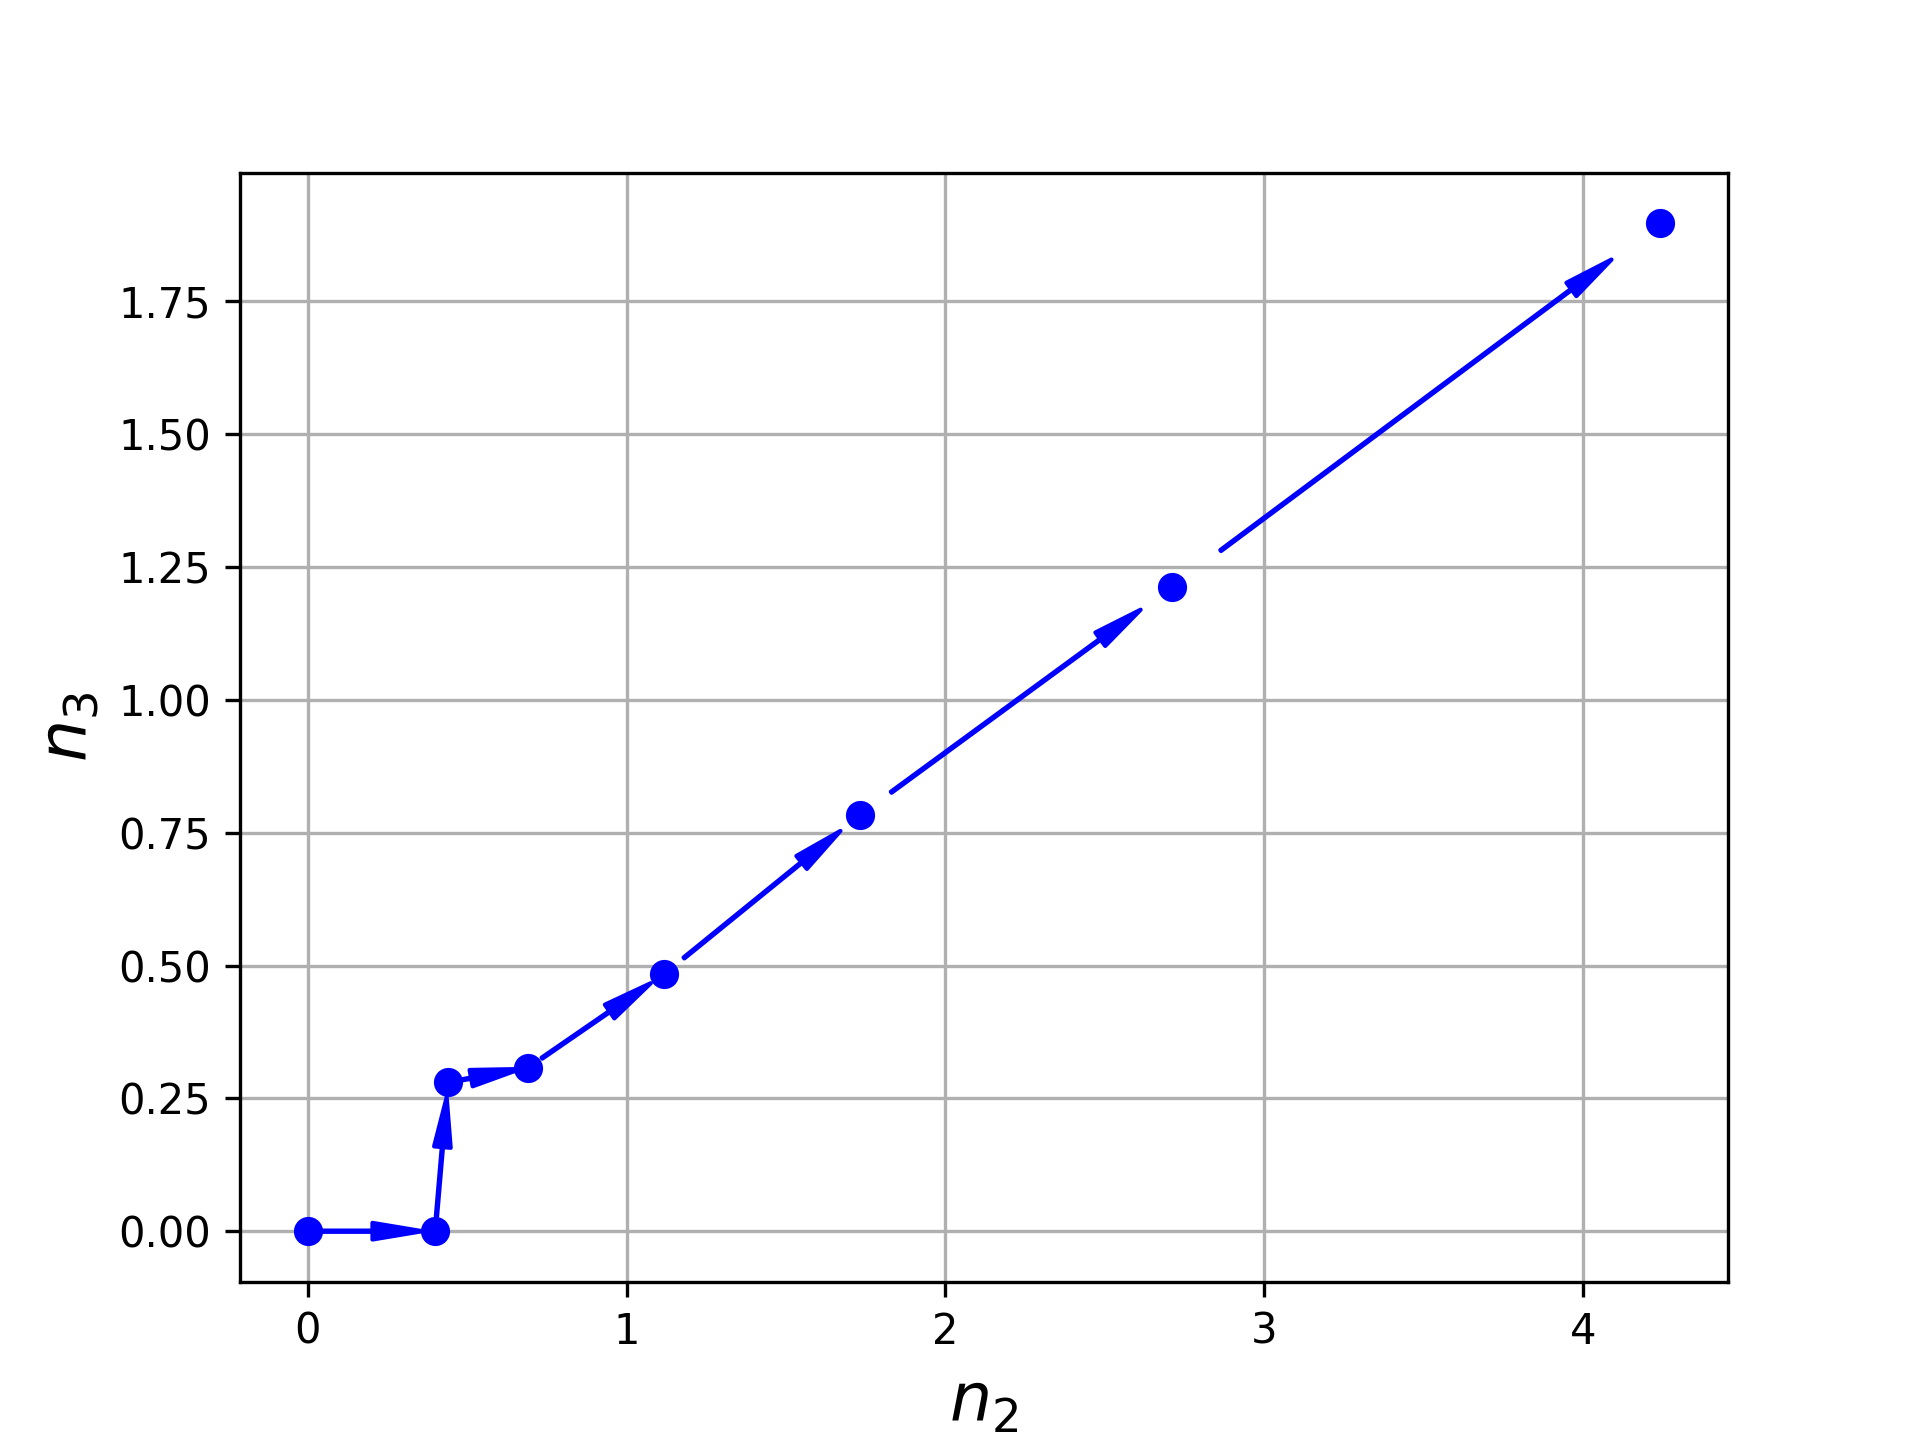
\includegraphics[width=0.7\textwidth]{project_n2_n3}	
	\end{center}
	\caption{Progression of the population of adult mice $n_2$ vs senior mice $n_3$. Each point represents the values of these two age groups in one generation and arrows have been added to show the direction in which changes are happening. After just a few generations, the progress goes along a very clear straight line that is determined by the dominant eigenvector of the leslie matrix. }
	\label{fig:leslie_phase}
\end{figure}

It is easy to prove that if a given vector $\mathbf{v}$ is an eigenvector of a matrix, so is any multiple $k \cdot\mathbf{v}$. This demonstration is left as an exercise. For those who feel ready for a bigger challenge, it is also possible to show why the dominant eigenvalue determines the final age structure. \textbf{Hint:} any vector can be written as a linear combination of the eigenvalues.

\subsection{Complex eigenvalues}

In some cases, a Leslie matrix does not behave as stated before. Lets see the following model describing the dynamics of a locust population. Locusts have three stages in their life cycle, just as the example before. The first stage, $n_1$, are the eggs, second stage individuals, $n_2$, are called hoppers since they are not yet able to fly. Finally, when an individual develops proper wings and the ability to fly, it is considered an adult, $n_3$.

The Leslie matrix for this case is:

\begin{equation}
L=\begin{pmatrix}
	0	&0	&1000	\\
	0.02	&0	&0	\\
	0	&0.05	&0	\\
\end{pmatrix}
\end{equation}

Inspection of the Leslie matrix already tells us a few things about the biology of locusts. First of all, the zero in the first row and second column tells us that hoppers are not yet sexually mature $f_2=0$ but adult locusts are extremely prolific with an average production of 1,000 eggs per individual. The survival rate of eggs is extremely low, with the survival rate of hopper being more that twice as high but still very low, with only 5\% of hoppers surviving until the adult stage.

\begin{figure*}
	\begin{center}
		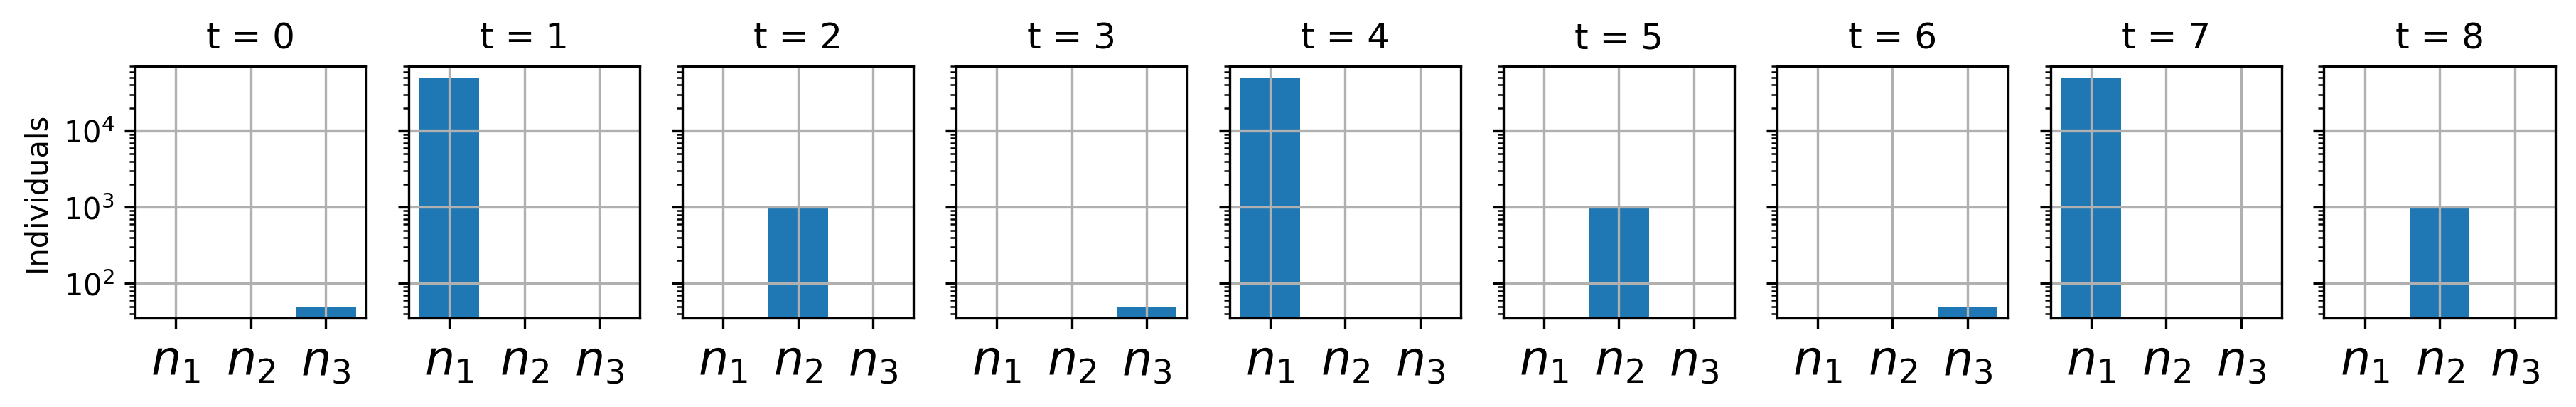
\includegraphics[width=\textwidth]{locusts_evol}
		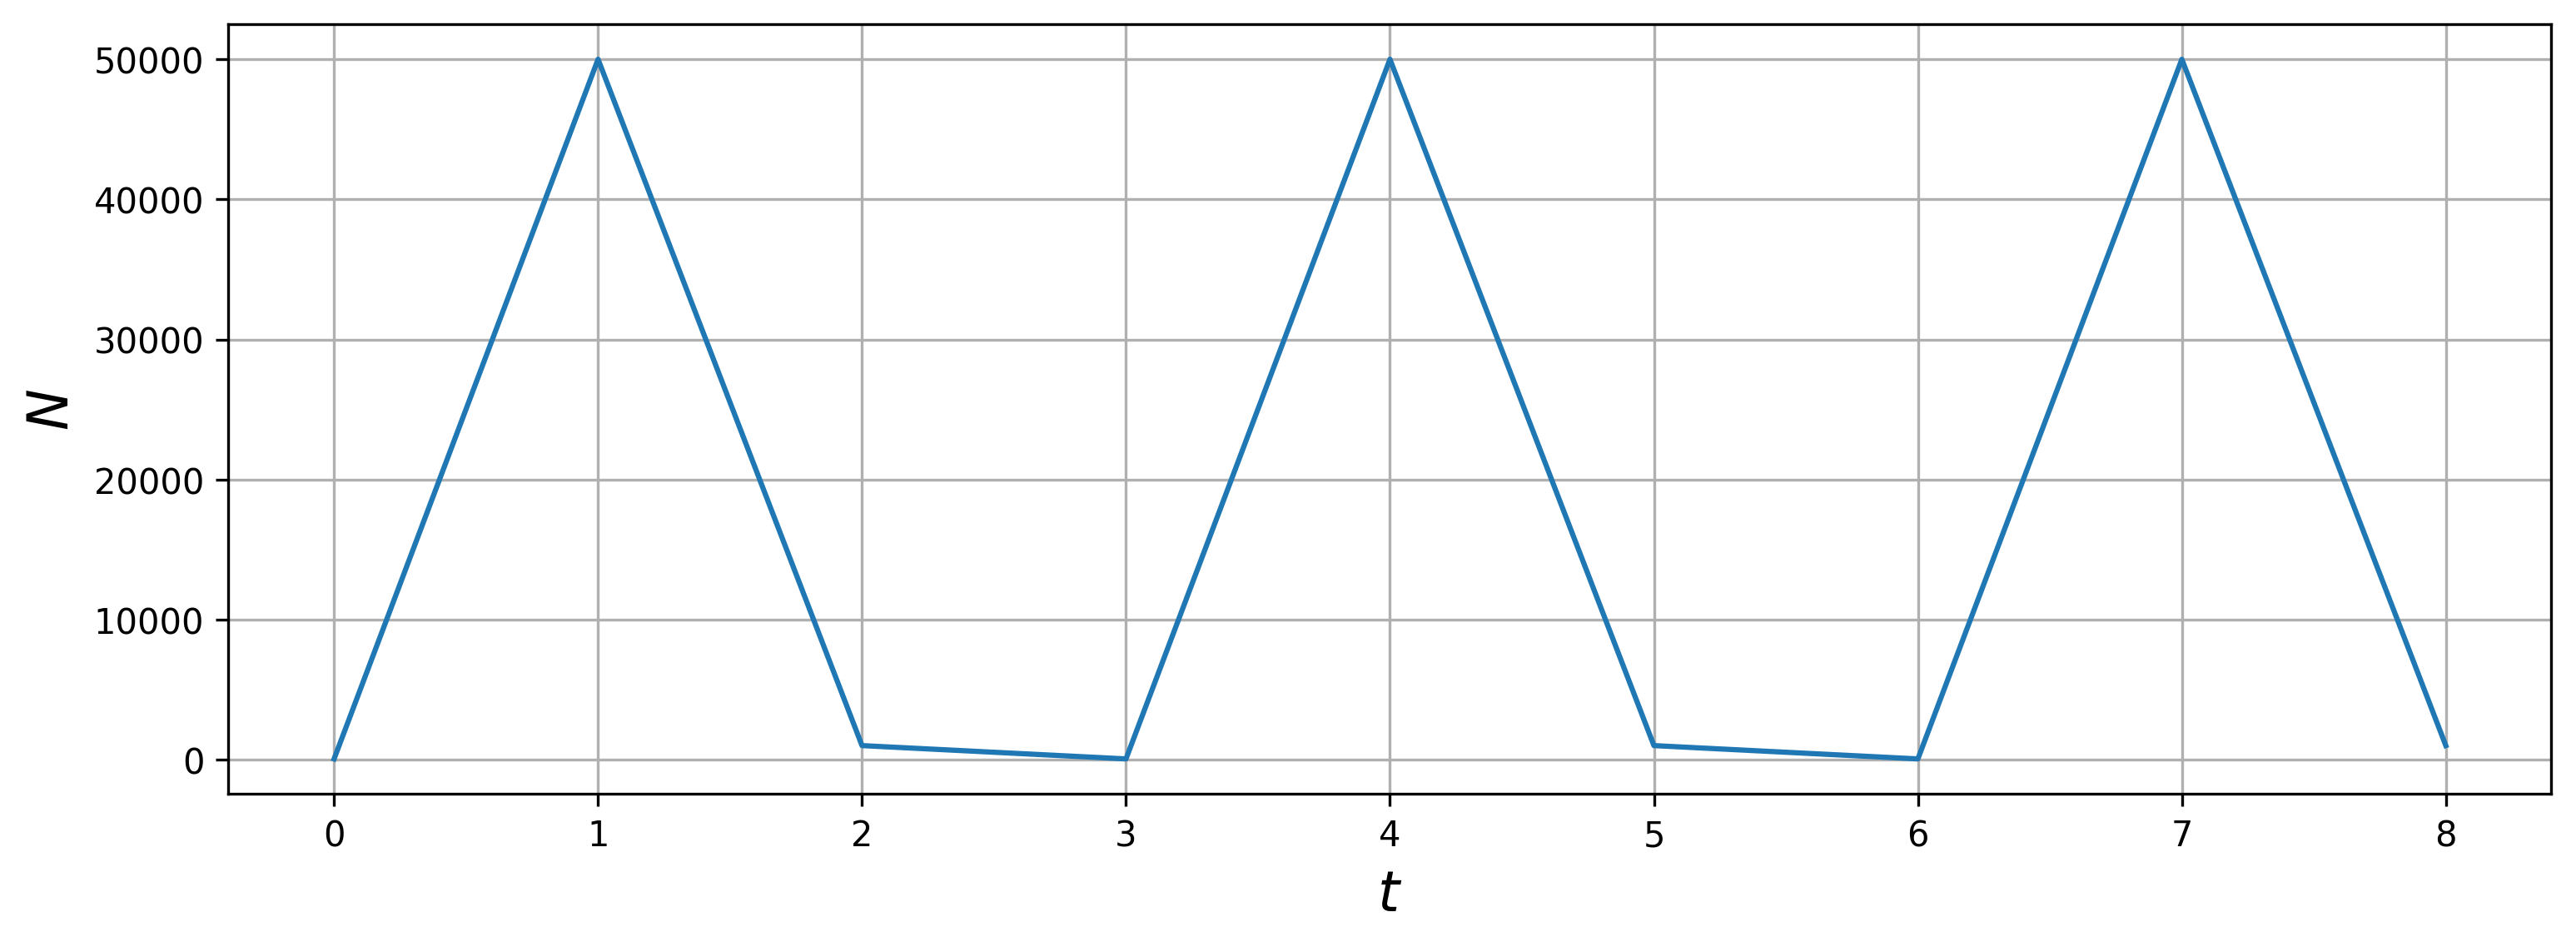
\includegraphics[width=\textwidth]{tot_locusts_evol}		
	\end{center}
	\caption{The upper graph shows the population structure as a bar graph for nine generations (y axis in log-coordinates). The figure below shows the total population for each generation (the sum of all three age groups). Unlike the previous case, we can clearly see an oscillating population.}
	\label{fig:Llocusts}
\end{figure*}

Simulating nine generations with this matrix, as can be seen in figure \ref{fig:Llocusts} shows a very different behavior. This population does not grow as before, but keeps oscillating instead. Moreover, the age structure does not remain fixed, it keeps switching between three different shapes.


\begin{figure}
	\begin{center}
		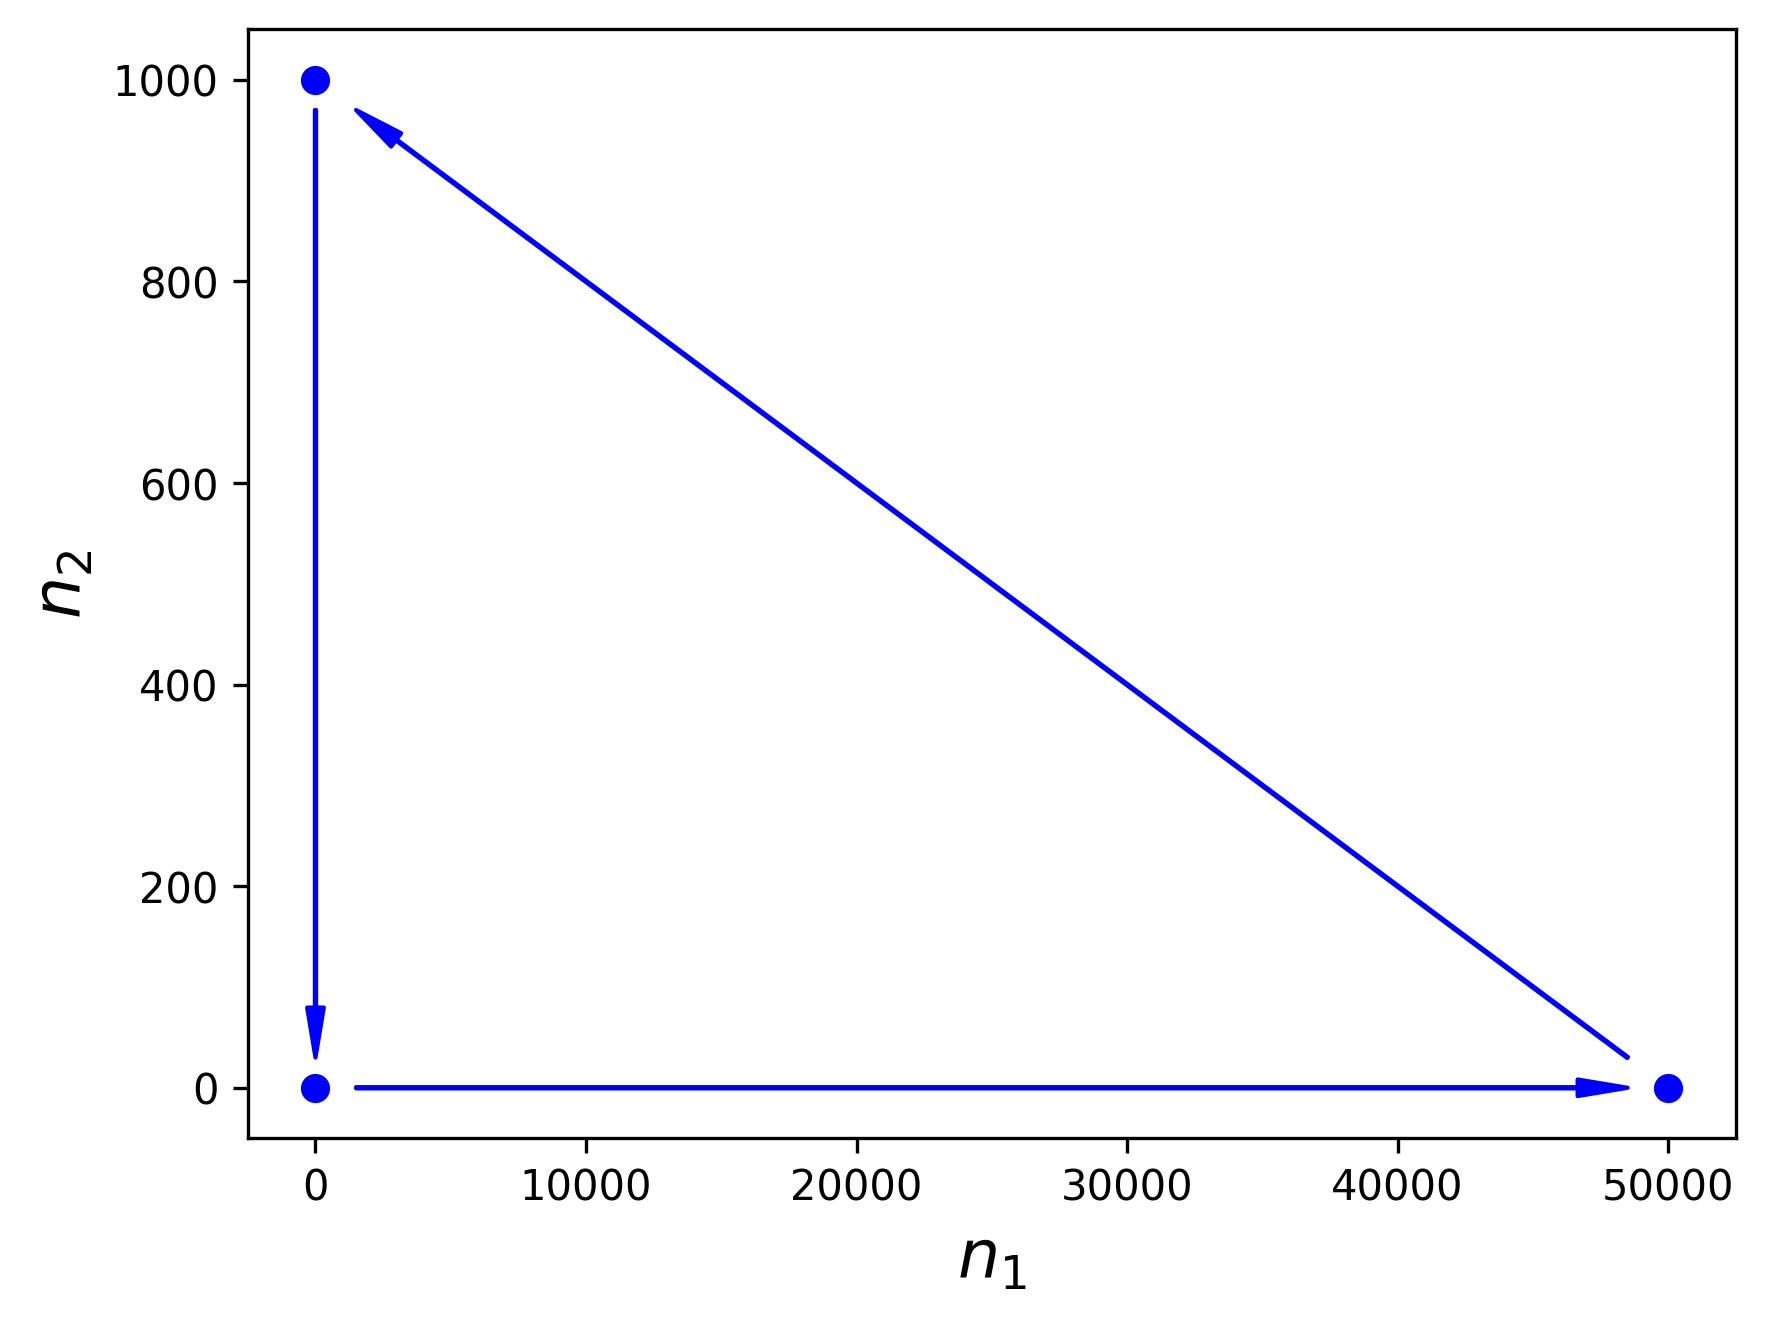
\includegraphics[width=0.7\textwidth]{locusts_phaseI}	
	\end{center}
	\caption{Progression of the population of eggs $n_1$ vs hoppers $n_2$. Each point represents the values of these two age groups in one generation and arrows have been added to show the direction in which changes are happening. Only three generations are shown since the third generation ends up exactly in the same position as the first, therefore repeating this cycle over and over }
	\label{fig:leslie_locust_phase}
\end{figure}

We can also view a projection of the amount of eggs and hoppers as we did with mice in figure \ref{fig:leslie_phase}. The result is a completely different behavior shown in figure \ref{fig:leslie_locust_phase}. It is noteworthy that periodic behaviors -- oscillations -- result in closed orbits in the phase space. 



\begin{figure*}
	\begin{center}
		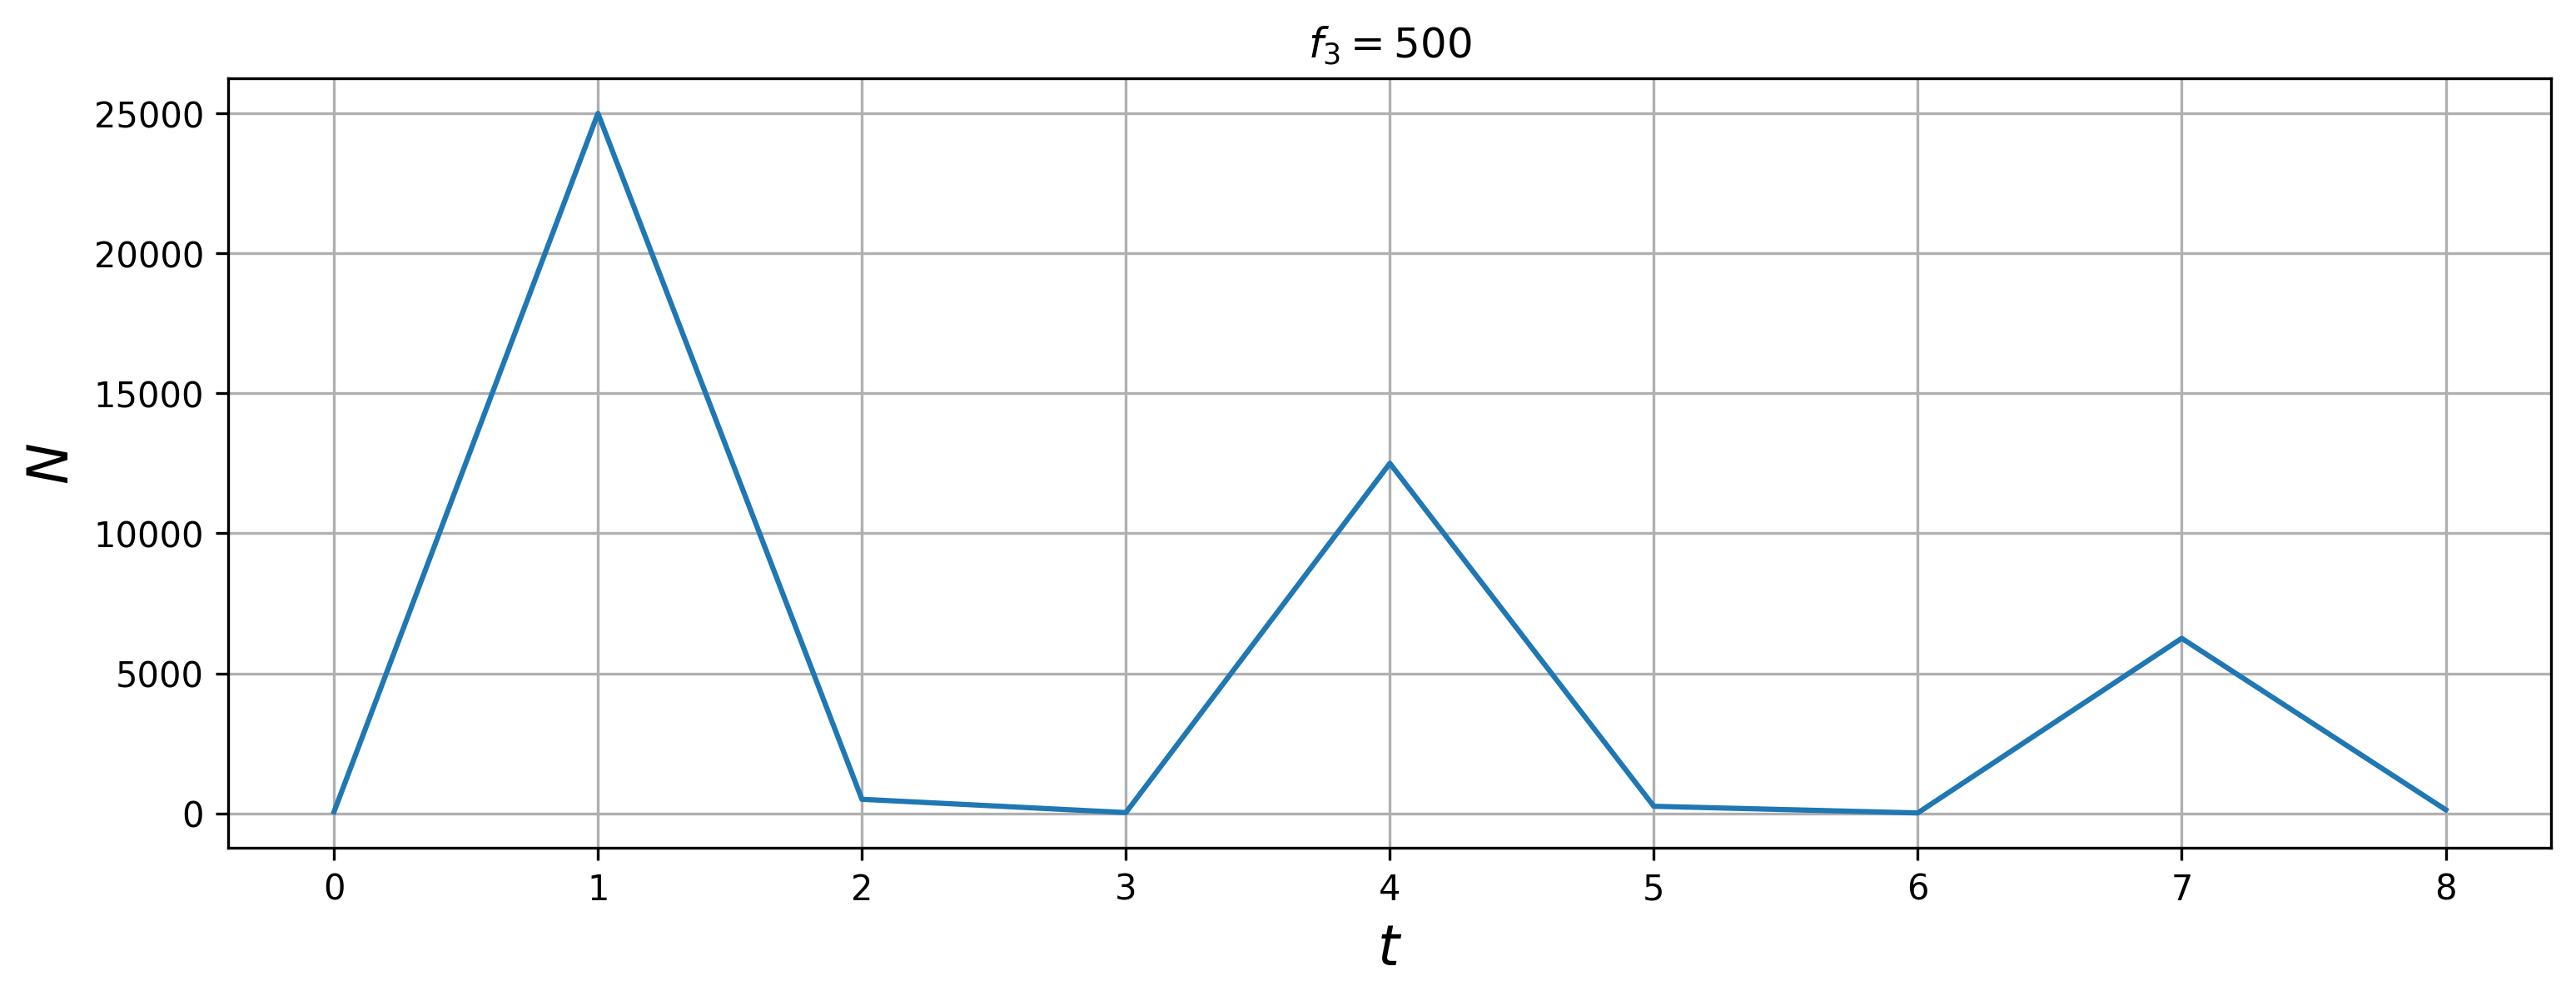
\includegraphics[width=\textwidth]{tot_locusts_evol_dec}
		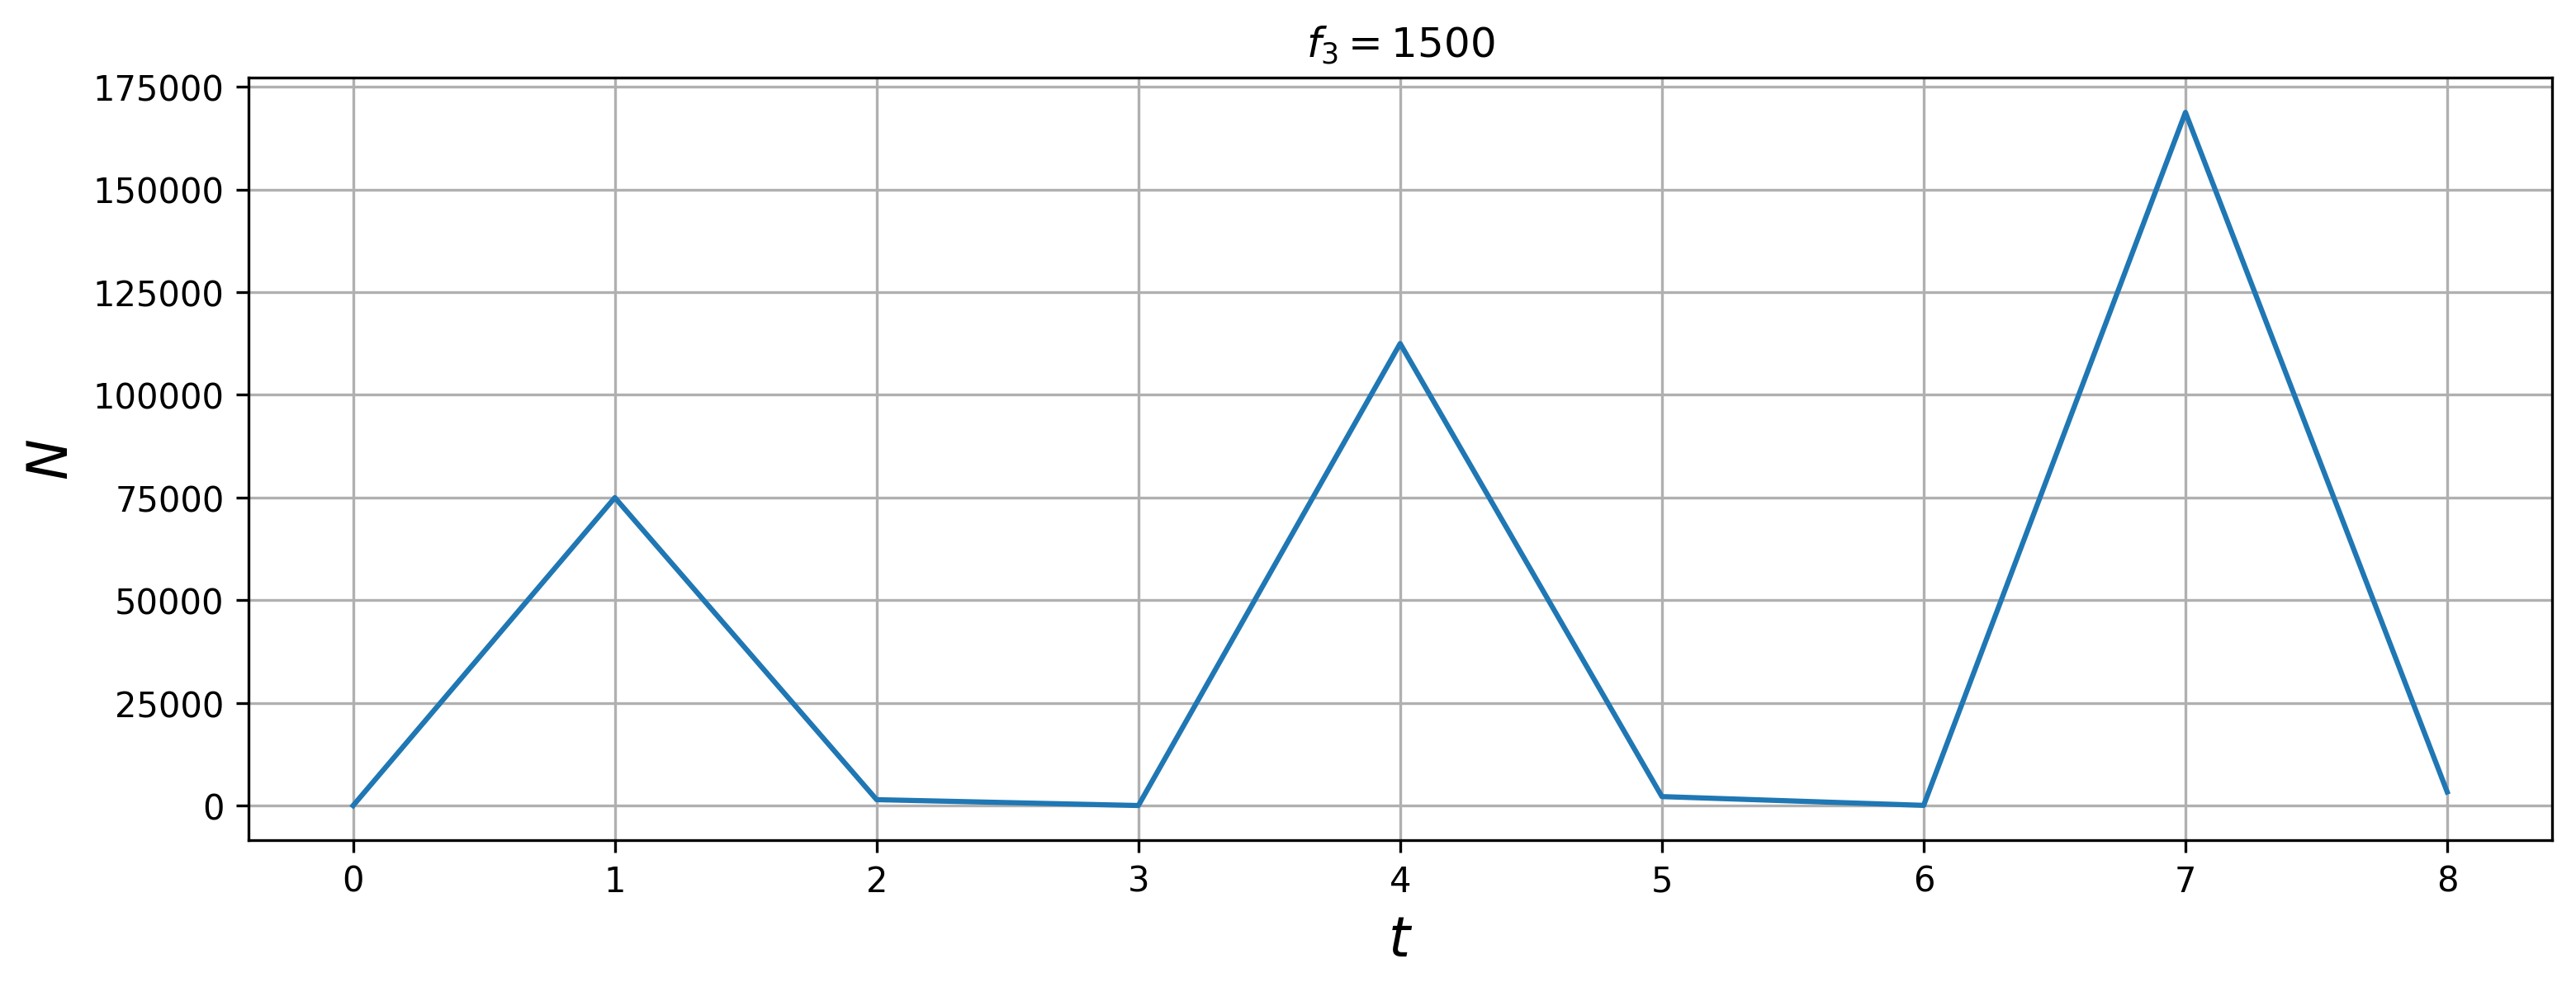
\includegraphics[width=\textwidth]{tot_locusts_evol_inc}
	\end{center}
	\caption{Evolution of the total number of locusts for different values of adult fecundity. At lower fecundities ($f_3 = 500$) the population exhibits damped oscillations until it eventually reaches extinction $N=0$. For higher fecundities $f_3 = 1,500$, the size of the population increases towards infinity. Obviously, the population will eventually collapse due to lack of resources.}
	\label{fig:Llocusts_stability}
\end{figure*}

Complex eigenvalues always result in oscillatory dynamics, but these oscillations are not always sustained. When the oscillations decrease in amplitude, the oscillation is said to be dampened and the system is said to be stable, because it is going towards a certain point where it will stay as time goes to infinity. If the oscillations have increased amplitude, the system will not be able to sustain the oscillation, and it is said to be unstable.

\begin{figure}
	\begin{center}
		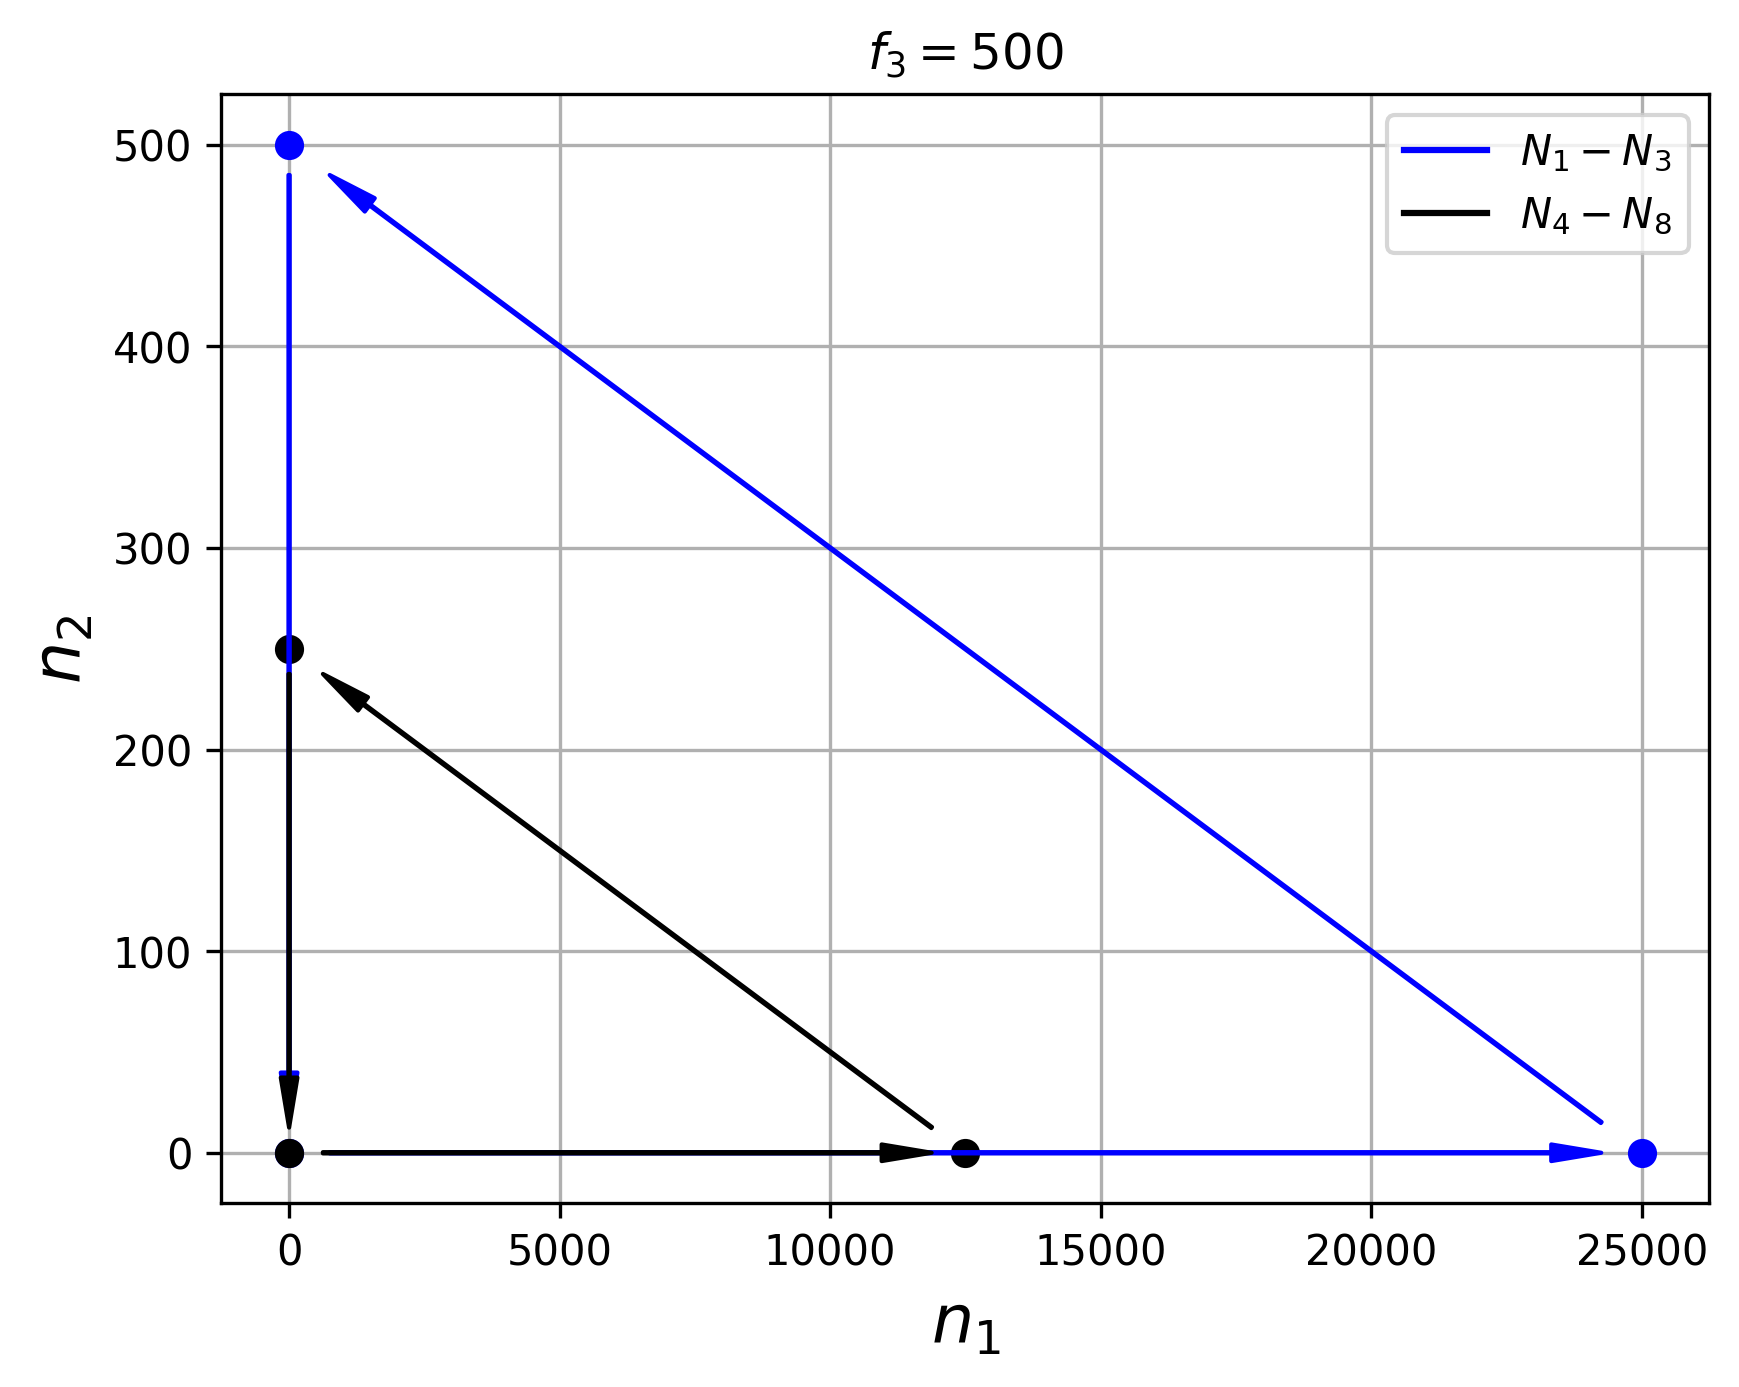
\includegraphics[width=0.45\textwidth]{locusts_phaseIdec}
		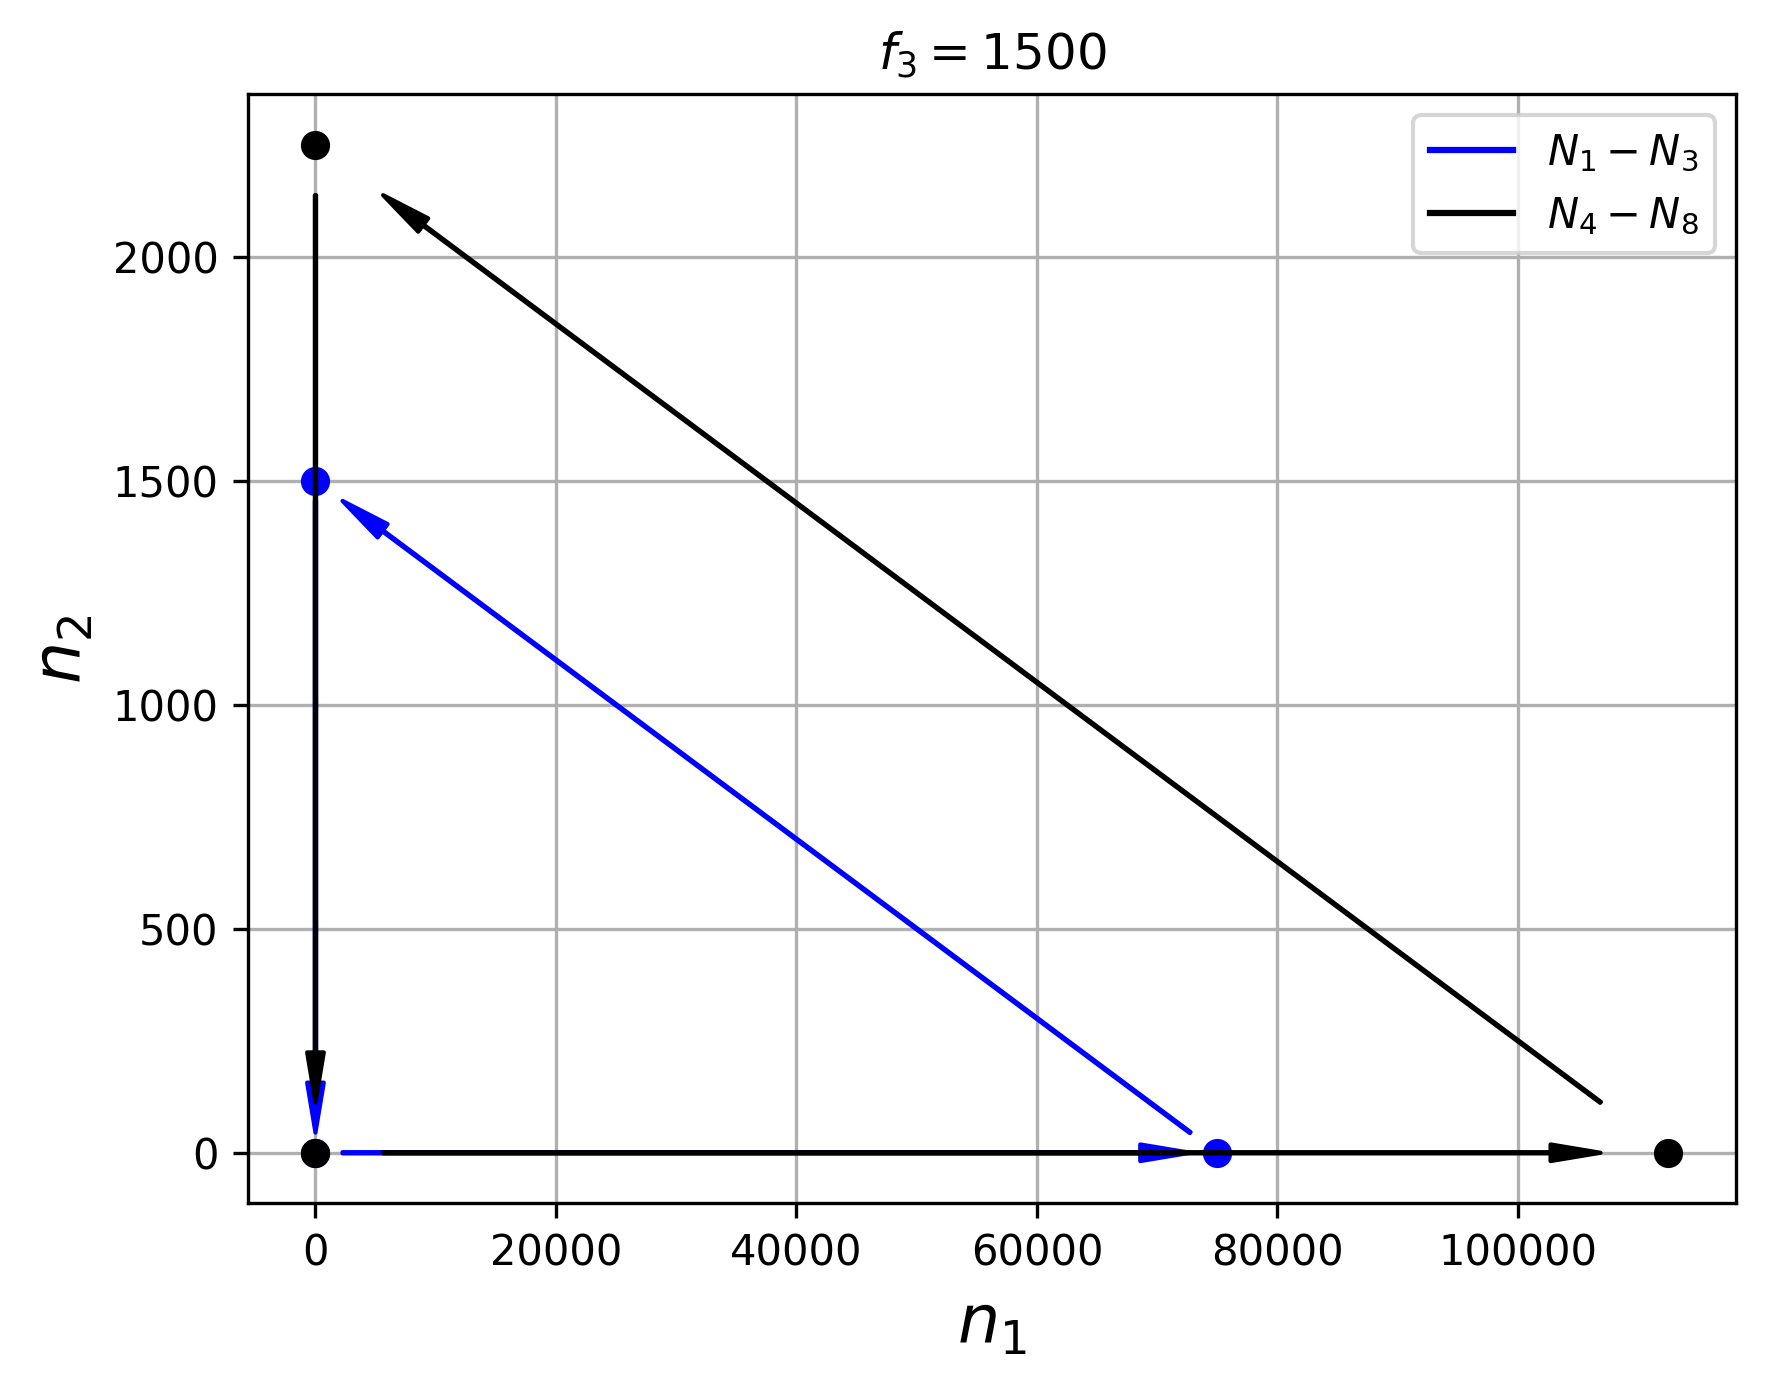
\includegraphics[width=0.45\textwidth]{locusts_phaseIinc}
	\end{center}
	\caption{Phase space representation (only 2D) for two different fecundities. The first three generations are displayed in blue and the next three in black to facilitate interpretation. At low fecundities the orbits are almost closed but every turn is smaller until the system reaches zero as $t \mapsto \infty$. At higher fecundity, however, oscillations become wider.}
	 
	\label{fig:Llocusts_stability_pp}
\end{figure}

\FloatBarrier